\section{Spectral Admissibility on the Binary Icosahedral Group $2I$}
  \label{sec:step5}

  \subsection{The group $2I$ and its place in the programme}
    \label{sec:step5-intro}

    The binary icosahedral group $2I$ is the double cover of the icosahedral
    rotation group $A_5 \cong \mathrm{PSL}(2,\mathbb{F}_5)$, and has order
    $|2I| = 120$.
    It is the largest finite subgroup of $\mathrm{SU}(2)$ and sits in the
    inclusion chain
    \begin{equation}
      Q_8 \subset 2I \subset \mathrm{SU}(2),
      \label{eq:chain}
    \end{equation}
    making it the natural next test case for the spectral admissibility
    programme.

    The irreducible representations of $2I$ are labelled by spin and have
    dimensions matching the low-spin content of $\mathrm{SU}(2)$:
    \begin{equation}
      \underbrace{1}_{\text{spin }0},\quad
      \underbrace{2,\,2'}_{\text{spin }\tfrac{1}{2}},\quad
      \underbrace{3,\,3'}_{\text{spin }1},\quad
      \underbrace{4,\,4'}_{\text{spin }\tfrac{3}{2}},\quad
      \underbrace{5}_{\text{spin }2},\quad
      \underbrace{6}_{\text{spin }\tfrac{5}{2}}.
      \label{eq:2I-irreps}
    \end{equation}
    Of these nine irreps, six are spin-type in the sense that they arise from
    restrictions of $\mathrm{SU}(2)$ representations.

  \subsection{Conjugacy classes and character table}
    \label{sec:step5-chars}

    The group $2I$ has nine conjugacy classes, enumerated by element order:
    \begin{center}
      \begin{tabular}{llcl}
        \hline
        Class & Order & Size & Notation                      \\
        \hline
        $1a$  & 1     & 1    & identity                      \\
        $2a$  & 2     & 1    & central element $-\mathbf{1}$ \\
        $3a$  & 3     & 20   &                               \\
        $4a$  & 4     & 30   &                               \\
        $5a$  & 5     & 12   &                               \\
        $5b$  & 5     & 12   & algebraic conjugate of $5a$   \\
        $6a$  & 6     & 20   &                               \\
        $10a$ & 10    & 12   &                               \\
        $10b$ & 10    & 12   & algebraic conjugate of $10a$  \\
        \hline
      \end{tabular}
    \end{center}
    The class sizes satisfy
    \[
      1+1+20+30+12+12+20+12+12 = 120.
    \]

    Writing $\varphi = (1+\sqrt{5})/2$ and
    $\bar\varphi = 1/\varphi = \varphi - 1 = (\sqrt{5}-1)/2$, the character
    values of the spin-type irreps are
    \begin{equation}
      \renewcommand{\arraystretch}{1.3}
      \begin{array}{l|rrrrrrrrr}
        & 1a & 2a & 3a & 4a & 5a & 5b & 6a & 10a & 10b \\
        \hline
        \chi_1 & 1 &  1 &  1 &  1 &  1 &  1 &  1 &  1 &  1 \\
        \chi_2 & 2 & -2 & -1 &  0 & \bar\varphi & -\varphi & 1 & \varphi & -\bar\varphi \\
        \chi_3 & 3 &  3 &  0 & -1 & \varphi & -\bar\varphi & 0 & -\bar\varphi & \varphi \\
        \chi_4 & 4 & -4 &  1 &  0 & -1 & -1 & -1 & 1 & 1 \\
        \chi_5 & 5 &  5 & -1 &  1 &  0 &  0 & -1 & 0 & 0 \\
        \chi_6 & 6 & -6 &  0 &  0 &  1 &  1 &  0 & -1 & -1
      \end{array}
      \label{eq:CT-2I}
    \end{equation}

  \subsection{Generating set: spinorial lift of fundamental rotations}
    \label{sec:step5-genset}

    A natural generating set for comparison with the $Q_8$ case is the union of
    the two order-10 conjugacy classes,
    \begin{equation}
      S = 10a \cup 10b,
      \qquad
      |S| = 24.
      \label{eq:S-2I}
    \end{equation}

    This choice is structurally motivated.
    The elements in the classes $10a$ and $10b$ are the spinorial lifts in $2I$
    of the order-5 rotations of the quotient group
    $A_5 \cong \mathrm{PSL}(2,\mathbb{F}_5)$.
    In this sense the construction parallels the $Q_8$ case, where the generators
    $\{\pm i,\pm j,\pm k\}$ arise as lifts of $\pi$-rotations in $SO(3)$.

    The set $S$ is inversion-symmetric, generates $2I$, and forms a union of
    conjugacy classes, ensuring that the adjacency operator acts by scalars
    on each irreducible representation.

    The hierarchy derived below is therefore established for this canonical
    spinorial generating set.
    Other generating sets may probe different structural questions and need
    not produce the same spectral ordering.

  \subsection{Adjacency eigenvalues and spectral hierarchy}
    \label{sec:step5-spectrum}

    For a generating set that is a union of conjugacy classes, the adjacency
    eigenvalue in the irreducible sector $\rho$ is
    \begin{equation}
      \mu_\rho
      = \frac{1}{\dim\rho}
      \sum_{C \subseteq S} |C|\,\chi_\rho(C).
      \label{eq:mu-formula-2I}
    \end{equation}
    For $S = 10a \cup 10b$, with both classes of size $12$, this gives
    \begin{equation}
      \renewcommand{\arraystretch}{1.4}
      \begin{array}{l|ccc}
        \text{Sector} &
        \mu_\rho &
        \lambda_\rho = 24 - \mu_\rho &
        A^{\max}_\rho = c_\chi/\sqrt{\lambda_\rho} \\
        \hline
        \chi_1\;(\text{trivial}) & 24 & 0  & \infty \\
        \chi_2\;(\text{spin-}{\tfrac{1}{2}}) & 6  & 18 & c_\chi/\sqrt{18} \\
        \chi_3\;(\text{spin-}1) & 4  & 20 & c_\chi/\sqrt{20} \\
        \chi_4\;(\text{spin-}{\tfrac{3}{2}}) & 6  & 18 & c_\chi/\sqrt{18} \\
        \chi_5\;(\text{spin-}2) & 0  & 24 & c_\chi/\sqrt{24} \\
        \chi_6\;(\text{spin-}{\tfrac{5}{2}}) & -4 & 28 & c_\chi/\sqrt{28}
      \end{array}
      \label{eq:2I-spectrum}
    \end{equation}

    The spectral ordering of the non-trivial spin-type sectors is therefore
    \begin{equation}
      \lambda_{1/2} = \lambda_{3/2} = 18
      < \lambda_1 = 20
      < \lambda_2 = 24
      < \lambda_{5/2} = 28.
      \label{eq:2I-ordering}
    \end{equation}

  \subsection{Algebraic origin: the golden ratio identity}
    \label{sec:step5-golden}

    For the spin-$\tfrac{1}{2}$ sector,
    \begin{equation}
      \mu_2
      = \frac{1}{2}\bigl(12\,\chi_2(10a) + 12\,\chi_2(10b)\bigr)
      = 6\bigl(\chi_2(10a)+\chi_2(10b)\bigr).
      \label{eq:mu2-computation}
    \end{equation}
    Using
    \begin{equation}
      \chi_2(10a)+\chi_2(10b)
      = \varphi + (-\bar\varphi)
      = \varphi - \bar\varphi
      = 1,
      \label{eq:golden-identity}
    \end{equation}
    we obtain
    \begin{equation}
      \mu_2 = 6.
      \label{eq:mu2-final}
    \end{equation}

    For the spin-$\tfrac{3}{2}$ sector, both classes have character $+1$:
    \begin{equation}
      \chi_4(10a)=\chi_4(10b)=1,
      \qquad
      \mu_4=\frac{12+12}{4}=6.
      \label{eq:mu4-computation}
    \end{equation}

  \subsection{Comparison with $Q_8$ and the strengthening hierarchy}
    \label{sec:step5-comparison}

    \begin{figure}[t]
      \centering
      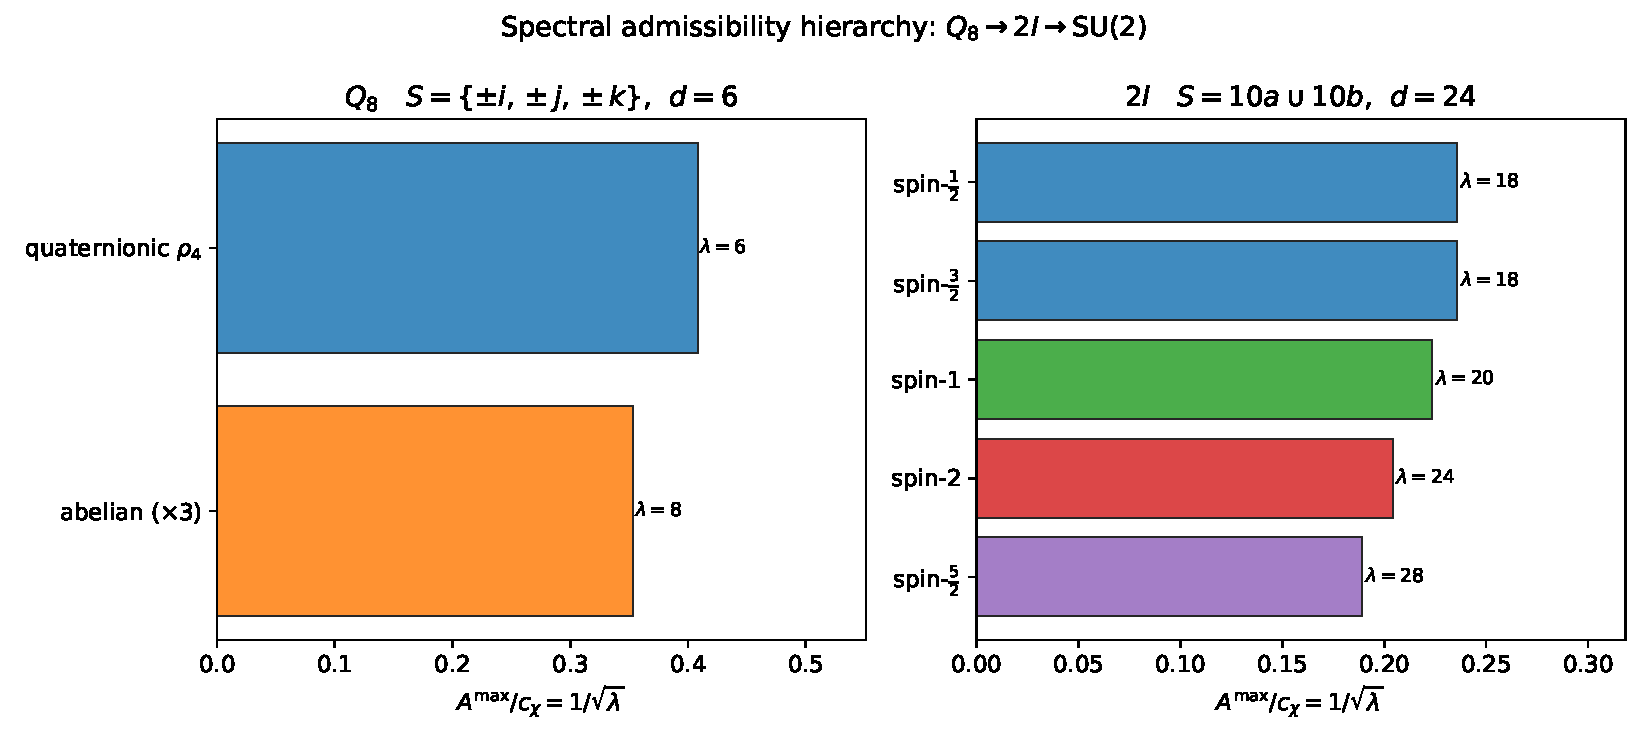
\includegraphics[width=0.95\textwidth]{fig3_hierarchy_Q8_vs_2I}
      \caption{
        Spectral admissibility hierarchy from $Q_8$ to $2I$.
        Left: on $Q_8$, the quaternionic sector has the smallest non-trivial
        Laplacian eigenvalue.
        Right: on $2I$ with generating set $S=10a\cup 10b$, the hierarchy
        resolves into the ordered spin-type sectors
        $\lambda_{1/2}=\lambda_{3/2}=18 < \lambda_1=20 < \lambda_2=24 <
        \lambda_{5/2}=28$.
        The comparison illustrates the sharpening of the admissibility
        hierarchy along the chain $Q_8 \subset 2I \subset \mathrm{SU}(2)$.
      }
      \label{fig:q8-2i-hierarchy}
    \end{figure}

    On $Q_8$ with $S=\{\pm i,\pm j,\pm k\}$,
    \begin{equation}
      \frac{A^{\max}_{\mathrm{best}}}{A^{\max}_{\mathrm{worst}}}
      = \sqrt{\frac{8}{6}}
      = \sqrt{\frac{4}{3}}
      \approx 1.155.
      \label{eq:Q8-ratio}
    \end{equation}

    On $2I$ with $S = 10a \cup 10b$, the corresponding ratio is
    \begin{equation}
      \frac{A^{\max}_{1/2}}{A^{\max}_{5/2}}
      = \sqrt{\frac{28}{18}}
      = \sqrt{\frac{14}{9}}
      \approx 1.247.
      \label{eq:2I-ratio}
    \end{equation}

    Thus the admissibility contrast increases from $Q_8$ to $2I$:
    \begin{equation}
      \sqrt{\frac{4}{3}}
      \approx 1.155
      \quad\longrightarrow\quad
      \sqrt{\frac{14}{9}}
      \approx 1.247.
      \label{eq:growing-hierarchy}
    \end{equation}

  \subsection{Physical interpretation: towards low-spin selection}
    \label{sec:step5-physics}

    On $Q_8$, the admissibility hierarchy separated the non-abelian sector from
    the abelian sectors.
    On $2I$, the hierarchy is resolved across several spin sectors:
    \begin{equation}
      \text{spin-}\tfrac{1}{2},\,\text{spin-}\tfrac{3}{2}
      \;\succ\;
      \text{spin-}1
      \;\succ\;
      \text{spin-}2
      \;\succ\;
      \text{spin-}\tfrac{5}{2},
      \label{eq:spin-ladder}
    \end{equation}
    where $\succ$ denotes a strictly larger admissibility window.

    The ordering is not strictly monotone in spin, since the
    spin-$\tfrac{1}{2}$ and spin-$\tfrac{3}{2}$ sectors are degenerate.
    Even so, the hierarchy is clearly biased toward lower spins.
